\chapter{Wstęp teoretyczny}

\section{Grafowa baza danych}

Projekt RevCommunity przyjmuje formę portalu społecznościowego bogatego w powiązania między różnymi jego elementami. Użytkownicy mogą obserwować produkty i subskrybować kanały innych użytkowników. Kategorie produktów mają strukturę drzewiastą. Taka specyfika systemu nasuwa pytanie, czy zastosowanie popularnego relacyjnego modelu danych jest najlepszym rozwiązaniem. Naszym zdaniem dużo korzystniejszym wyjściem jest zastosowanie nowej szybko rozwijającej się technologii grafowej bazy danych. W porównaniu do RBD model grafowy bardziej naturalnie reprezentuje rzeczywistość. Dużo łatwiej odwzorować struktury obiektowe na węzły i łuki grafu niż tabele powiązane kluczami obcymi, czy dodatkowymi tabelami. Dlatego często stosowana jest warstwa ORM jako pośrednicząca między obiektowymi językami programowania, a RBD. Duże znaczenie ma tutaj wydajność obu podejść. Grafowe bazy danych okazują się niebywale wydajne przy zapytaniach opierających się na połączeniach między elementami. RBD wręcz przeciwnie, ponieważ każde zapytanie odwołujące się do powiązanych tabel wymaga kosztownego połączenia kilku tabel. Model grafowy rozwiązuje również problem przechowywania struktur drzewiastych.
Odnośnie samej zasady działania grafowych baz danych możemy powiedzieć, że dane są reprezentowane przez węzły i łuki. Węzły to instancje obiektów(odpowiedniki rekordów w RBD). Posiadają atrybuty i mogą być powiązane z innymi węzłami. Łuki natomiast reprezentują relacje między węzłami. Każdy łuk musi posiadać węzeł początkowy i końcowy, oraz etykietę oznaczającą typ relacji. Możemy również definiować atrybuty powiązań, czyli tak zwane bogate relacje (rich relationship). Ze względu na kierunek możemy wyróżnić trzy rodzaje łuków:
\begin{itemize}
\item Wyjściowe
\item Wejściowe
\item Nieskierowane
\end{itemize}


\begin{figure}[h]
	\centering
	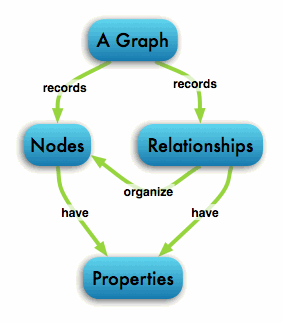
\includegraphics[scale=1]{images/graphdb.png}
	\caption{Schemat działania grafowej bazy danych}
\end{figure}




